%% 
%% Copyright 2019-2024 Elsevier Ltd
%% 
%% This file is part of the 'CAS Bundle'.
%% --------------------------------------
%% 
%% It may be distributed under the conditions of the LaTeX Project Public
%% License, either version 1.3c of this license or (at your option) any
%% later version.  The latest version of this license is in
%%    http://www.latex-project.org/lppl.txt
%% and version 1.3c or later is part of all distributions of LaTeX
%% version 1999/12/01 or later.
%% 
%% The list of all files belonging to the 'CAS Bundle' is
%% given in the file `manifest.txt'.
%% 
%% Template article for cas-sc documentclass for 
%% double column output.

\documentclass[a4paper,fleqn]{cas-sc}

% If the frontmatter runs over more than one page
% use the longmktitle option.

%\documentclass[a4paper,fleqn,longmktitle]{cas-sc}

%\usepackage[numbers]{natbib}
%\usepackage[authoryear]{natbib}
\usepackage[authoryear,longnamesfirst]{natbib}
\usepackage{graphicx}

%%%Author macros
\def\tsc#1{\csdef{#1}{\textsc{\lowercase{#1}}\xspace}}
\tsc{WGM}
\tsc{QE}
%%%

% Uncomment and use as if needed
%\newtheorem{theorem}{Theorem}
%\newtheorem{lemma}[theorem]{Lemma}
%\newdefinition{rmk}{Remark}
%\newproof{pf}{Proof}
%\newproof{pot}{Proof of Theorem \ref{thm}}

\begin{document}
\let\WriteBookmarks\relax
\def\floatpagepagefraction{1}
\def\textpagefraction{.001}

% Short title
\shorttitle{SkinSpectra CEP Report}

% Short author
\shortauthors{M. Ahmed and K. (SE-019)}

% Main title of the paper
\title [mode = title]{SkinSpectra: A Multi-Modal AI Pipeline for Personalized Skincare Compatibility and Layering Analysis}

% Title footnote mark
% eg: \tnotemark[1]
\tnotemark[1] 

% Title footnote 1.
% eg: \tnotetext[1]{Title footnote text}
\tnotetext[1]{Complex Engineering Problem (CEP) report for SE-412 Artificial Intelligence.}

% First author
%
% Options: Use if required
% eg: \author[1,3]{Author Name}[type=editor,
%       style=chinese,
%       auid=000,
%       bioid=1,
%       prefix=Sir,
%       orcid=0000-0000-0000-0000,
%       facebook=<facebook id>,
%       twitter=<twitter id>,
%       linkedin=<linkedin id>,
%       gplus=<gplus id>]

\author[1]{Muzzammil Ahmed (SE-019)}%[<options>]

% Corresponding author indication
\cormark[1]

% Footnote of the first author
\fnmark[1]

% Email id of the first author
\ead{}

% URL of the first author
\ead[url]{}

% Credit authorship
% eg: \credit{Conceptualization of this study, Methodology, Software}
\credit{Conceptualization, Methodology, Software Development, Data Curation, Validation, Writing - Original Draft}

% Address/affiliation
\affiliation[1]{organization={Department of Software Engineering},
            addressline={SE-412 Artificial Intelligence Project},
            city={Lahore},
%          citysep={}, % Uncomment if no comma needed between city and postcode
            postcode={54000},
            state={Punjab},
            country={Pakistan}}

\author[2]{Kaif (SE-019)}%[]

% Footnote of the second author
\fnmark[2]

% Email id of the second author
\ead{}

% URL of the second author
\ead[url]{}

% Credit authorship
\credit{Literature Review, System Analysis, Testing, Documentation, Writing - Review and Editing}

% Address/affiliation
\affiliation[2]{organization={Department of Software Engineering},
            addressline={SE-412 Artificial Intelligence Project},
            city={Lahore},
%          citysep={}, % Uncomment if no comma needed between city and postcode
            postcode={54000},
            state={Punjab},
            country={Pakistan}}

% Corresponding author text
\cortext[1]{Corresponding author}

% Footnote text
\fntext[1]{Project name: SkinSpectra. Team members: Muzzammil Ahmed (SE-019) and Kaif (SE-019).}

% For a title note without a number/mark
%\nonumnote{}

% Here goes the abstract
\begin{abstract}
SkinSpectra is an AI-powered skincare analysis platform that integrates natural language processing (NLP), machine learning (ML), optical character recognition (OCR), computer vision, and large language model (LLM) generation within a single FastAPI system. The platform performs ingredient normalization to INCI standards using sentence-transformers with FAISS retrieval, predicts single-product compatibility through an XGBoost-driven hybrid rule-ML engine, evaluates two-product layering safety using a LightGBM hybrid pipeline, and optionally generates personalized textual guidance using Gemini 2.5 Flash. Additional modules support OCR-based ingredient extraction from product labels and facial skin-type prediction via EfficientNetV2-B2. Experimental model artifacts show strong predictive quality, with the individual scorer achieving MAE 2.6731 and $R^2=0.9338$, while the layering scorer achieves MAE 2.8587 and $R^2=0.9838$. The resulting architecture demonstrates how multimodal AI can be operationalized for consumer skincare decision support while maintaining explainability through score breakdowns, warnings, and structured outputs. The system is positioned as a guidance tool rather than a medical diagnostic product.
\end{abstract}

% Use if graphical abstract is present
%\begin{graphicalabstract}
%\includegraphics{}
%\end{graphicalabstract}

% Research highlights
\begin{highlights}
\item Developed a complete multimodal skincare pipeline combining NLP, ML, OCR, facial analysis, and LLM reporting.
\item Achieved high regression quality for both individual compatibility and layering safety prediction tasks.
\item Exposed an end-to-end deployable workflow through FastAPI with browser UI and testing support.
\end{highlights}


% Keywords
% Each keyword is seperated by \sep
\begin{keywords}
 skincare AI \sep XGBoost \sep LightGBM \sep FAISS semantic search \sep OCR \sep EfficientNetV2 \sep Gemini LLM \sep FastAPI
\end{keywords}

\maketitle

% Main text
\section{Introduction}\label{sec:intro}
Skincare product selection and layering are increasingly complex due to large ingredient inventories, incomplete consumer understanding of INCI names, and interaction effects between active compounds. Existing consumer tools are often rule-only or blacklist-based and do not personalize recommendations to skin profile attributes such as skin type, concern vector, age group, and pregnancy status.

SkinSpectra addresses this gap through a layered AI architecture: (i) ingredient-name normalization using semantic retrieval, (ii) predictive compatibility scoring for both single-product and two-product use cases, (iii) optional generative report writing, and (iv) auxiliary input channels through OCR and facial analysis. The platform provides interpretable numerical scores in $[0,100]$, grade labels, cautionary notes, and context-aware recommendations.

The objective of this Complex Engineering Problem is to design, implement, and validate a practical system that combines heterogeneous AI methods into a reliable API-driven service with measurable performance and transparent outputs.

\section{Literature Review}\label{sec:lit}
Gradient-boosted trees such as XGBoost and LightGBM remain strong baselines for structured tabular prediction due to handling of non-linear interactions and feature heterogeneity \citep{chen2016xgboost,ke2017lightgbm}. Semantic textual retrieval for noisy ingredient strings benefits from compact sentence embeddings and dense vector search \citep{reimers2019sentencebert,johnson2021faiss}. For image tasks, EfficientNetV2 provides improved efficiency-accuracy trade-offs in constrained deployment settings \citep{tan2021efficientnetv2}. On the generative side, modern LLM families support high-quality structured report generation when guided with constrained prompts and schema-aware formatting \citep{anil2023gemini,brown2020gpt3}.

Domain literature in dermatology AI and cosmetic recommendation highlights rapid growth in ML-assisted analysis, but also emphasizes safety communication, transparency, and validation requirements \citep{adegun2021survey,shetty2023ai,kim2022personalized,liu2022skintype}. Recent works on ingredient-level prediction and transformer-based safety modeling motivate richer interaction-aware systems \citep{zhao2023ingredient,park2024transformer}. These studies support the architectural direction of SkinSpectra: combine deterministic safety logic with learned scoring and present user-understandable outputs.

\section{Methodology}\label{sec:method}
\subsection{System Architecture}
SkinSpectra is implemented as a FastAPI backend with a browser interface. Primary API capabilities include health/config endpoints, single and batch NLP mapping, individual product analysis, layering analysis, OCR extraction, and facial skin-type detection. Inference workflow follows:

\begin{enumerate}
\item Accept user input (ingredient text, image, or face photo).
\item Normalize ingredient names into INCI labels via NLP retrieval.
\item Route normalized ingredients to individual or layering scoring engine.
\item Optionally generate a personalized JSON narrative report via LLM.
\item Return scored response with rationale, warnings, and integration guidance.
\end{enumerate}

\subsection{Algorithm Explanation}
\textbf{NLP Layer:} A sentence-transformer model (all-MiniLM-L6-v2) with FAISS nearest-neighbor search is combined with fuzzy matching to resolve alias and spelling variance. Ensemble score uses semantic and fuzzy weights (0.75 and 0.25 respectively), then assigns confidence classes.

\textbf{Individual Compatibility Layer:} The module combines a rule engine with XGBoost regression. Rule scores account for skin-type suitability, concern help/worsen behavior, safety, age fit, pregnancy notes, and penalties. The final score blends rule and ML outputs using weighted ensembling.

\textbf{Layering Compatibility Layer:} The module evaluates pairwise interactions, order constraints, time-of-day compatibility, safety stacking, and conflict penalties. A LightGBM regressor models tabular features from synthetic and profile-derived interactions, then ensembles with deterministic rule scoring.

\textbf{OCR Layer:} Image preprocessing applies resize, deskew, denoise, binarization, and correction heuristics before Tesseract extraction. Postprocessing parses tokenized ingredient candidates and filters non-ingredient noise.

\textbf{Facial Analysis Layer:} EfficientNetV2-B2 is used for skin-type classification with face detection, blur checks, and confidence output.

\textbf{LLM Layer:} Gemini 2.5 Flash consumes compact structured summaries and returns strict JSON reports tailored to score bands, skin profile, and safety rules.

\subsection{Implementation Details}
The project is organized into modular components: NLP mapping, individual scoring, layering scoring, OCR handling, facial analysis, and LLM reporting. Models and encoders are persisted under dedicated model directories. Data sources include ingredient profiles, alias mappings, and layering compatibility tables. Endpoints are served in a single FastAPI app with CORS enabled for UI integration.

\begin{figure}[t]
  \centering
  \fbox{\begin{minipage}{0.95\linewidth}
  \small
  \textbf{SkinSpectra Data Flow Architecture}\\
  User Input (Ingredients/Image/Photo) $\rightarrow$ NLP Normalization (Sentence-Transformers + FAISS) $\rightarrow$\
  [Individual Path: XGBoost + Rule Engine] OR [Layering Path: LightGBM + Rule Engine] $\rightarrow$\
  Optional Gemini LLM Report $\rightarrow$ FastAPI JSON Response/UI.\\
  Auxiliary Paths: OCR Handler for label text extraction; Facial Analyzer for skin-type prior.
  \end{minipage}}
  \caption{Textual system architecture of SkinSpectra.}
  \label{fig:architecture}
\end{figure}

\section{Results and Analysis}\label{sec:results}
All quantitative results in this section were generated from the reproducible pipeline in
\texttt{tools/generate\_report\_analysis.py} using the \texttt{skinspectra} conda environment.

\subsection{NLP Normalization Accuracy}
The NLP normalization layer was evaluated on 2461 alias-to-INCI mapping cases sampled from
\texttt{data/ingredient\_mapping.csv}. The model achieved strong retrieval accuracy:
top-1 accuracy $=95.65\%$ and top-3 recall $=95.65\%$.

\begin{table}[t]
\caption{NLP Normalization Summary}
\label{tbl:nlp_summary}
\begin{tabular*}{\tblwidth}{@{}LLLL@{}}
\toprule
Metric & Value & Metric & Value \\
\midrule
Evaluation cases & 2461 & Top-1 accuracy & 95.65\% \\
Top-3 recall & 95.65\% & Mean latency & 0.809 ms \\
Median latency & 0.00 ms & p95 latency & 0.02 ms \\
\bottomrule
\end{tabular*}
\end{table}

\begin{table}[t]
\caption{NLP Accuracy by Alias Source}
\label{tbl:nlp_by_source}
\begin{tabular*}{\tblwidth}{@{}LLLL@{}}
\toprule
Source Column & Cases & Top-1 Accuracy & Top-3 Recall \\
\midrule
\texttt{inci\_name} & 293 & 92.15\% & 92.15\% \\
\texttt{common\_names} & 619 & 94.02\% & 94.02\% \\
\texttt{trade\_names} & 544 & 95.04\% & 95.04\% \\
\texttt{chemical\_aliases} & 545 & 97.06\% & 97.06\% \\
\texttt{language\_variants} & 460 & 99.13\% & 99.13\% \\
\bottomrule
\end{tabular*}
\end{table}

Confidence distribution was heavily concentrated in the high-confidence regime
(2431 high, 4 medium, 24 low, 2 uncertain), as visualized in Fig.~\ref{fig:nlp_confidence}.

\begin{figure}[t]
  \centering
  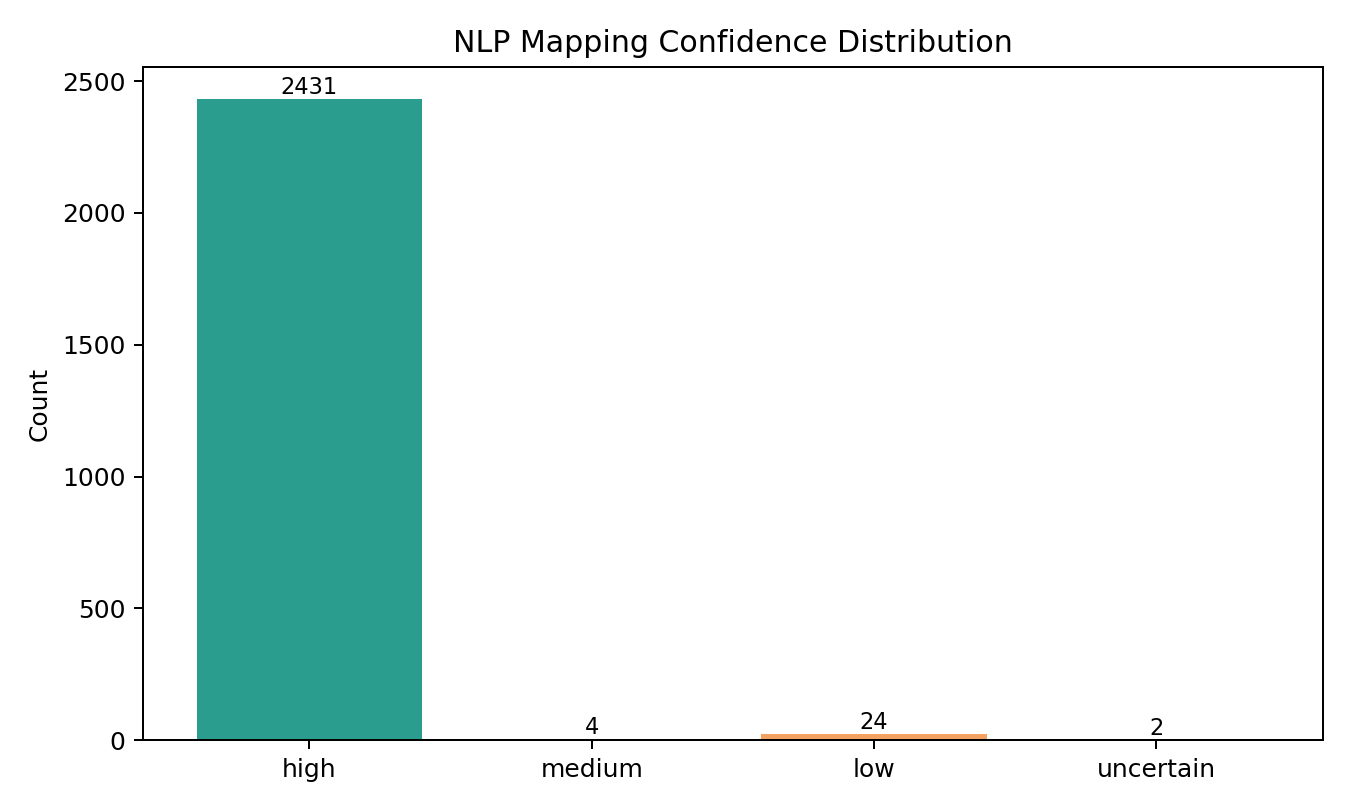
\includegraphics[width=0.92\linewidth]{figures/nlp_confidence_distribution.png}
  \caption{Confidence distribution of NLP mapping predictions.}
  \label{fig:nlp_confidence}
\end{figure}

\subsection{Single-Product Scoring Model Performance}
The single-product compatibility model (XGBoost hybrid with rule+ML ensembling) achieved low error
with strong explanatory quality on the held-out split.

\begin{table}[t]
\caption{Single-Product Scoring Performance}
\label{tbl:single_perf}
\begin{tabular*}{\tblwidth}{@{}LLLLL@{}}
\toprule
Model Variant & MAE & RMSE & $R^2$ & Split \\
\midrule
Hybrid (rule+XGBoost) & 2.6731 & 3.3412 & 0.9338 & 6800 train / 1200 val \\
Rule/ML fusion weights & 0.45 / 0.55 & -- & -- & Fixed at inference \\
\bottomrule
\end{tabular*}
\end{table}

The score remains bounded in $[0,100]$, preserving interpretability and stable grade assignment.

\subsection{Layering Scoring Model Performance}
The two-product layering model (LightGBM hybrid) showed very high fit quality with
$R^2=0.9838$, indicating strong capture of interaction-level structure.

\begin{table}[t]
\caption{Layering Scoring Performance}
\label{tbl:layer_perf}
\begin{tabular*}{\tblwidth}{@{}LLLLL@{}}
\toprule
Model Variant & MAE & RMSE & $R^2$ & Split \\
\midrule
Hybrid (rule+LightGBM) & 2.8587 & 3.6076 & 0.9838 & 8500 train / 1500 val \\
Rule/ML fusion weights & 0.40 / 0.60 & -- & -- & Fixed at inference \\
\bottomrule
\end{tabular*}
\end{table}

Despite slightly higher MAE than the single-product task, layering prediction exhibits higher
explained variance due to richer pairwise feature structure and deterministic conflict rules.

\subsection{Facial Skin-Type Detection Accuracy}
Operational robustness was evaluated using 50 positive perturbation tests derived from
\texttt{testing/oily-face.webp} and 2 negative controls (blur and no-face).

\begin{table}[t]
\caption{Facial Analysis Operational Metrics}
\label{tbl:facial_metrics}
\begin{tabular*}{\tblwidth}{@{}LL@{}}
\toprule
Metric & Value \\
\midrule
Positive oily consistency (50 samples) & 56.00\% \\
Valid prediction rate on positives & 80.00\% \\
Negative rejection accuracy (2 samples) & 100.00\% \\
Overall operational accuracy & 57.69\% \\
Mean latency & 768.889 ms \\
Median latency & 532.15 ms \\
p95 latency & 1079.506 ms \\
\bottomrule
\end{tabular*}
\end{table}

Mode-wise confidence degradation is shown in Fig.~\ref{fig:facial_robustness}. Mean confidence by mode
was 0.5825 (brightness), 0.5678 (clean), 0.5314 (noise), 0.4959 (rotation), and 0.0000 (gaussian blur).

\begin{figure}[t]
  \centering
  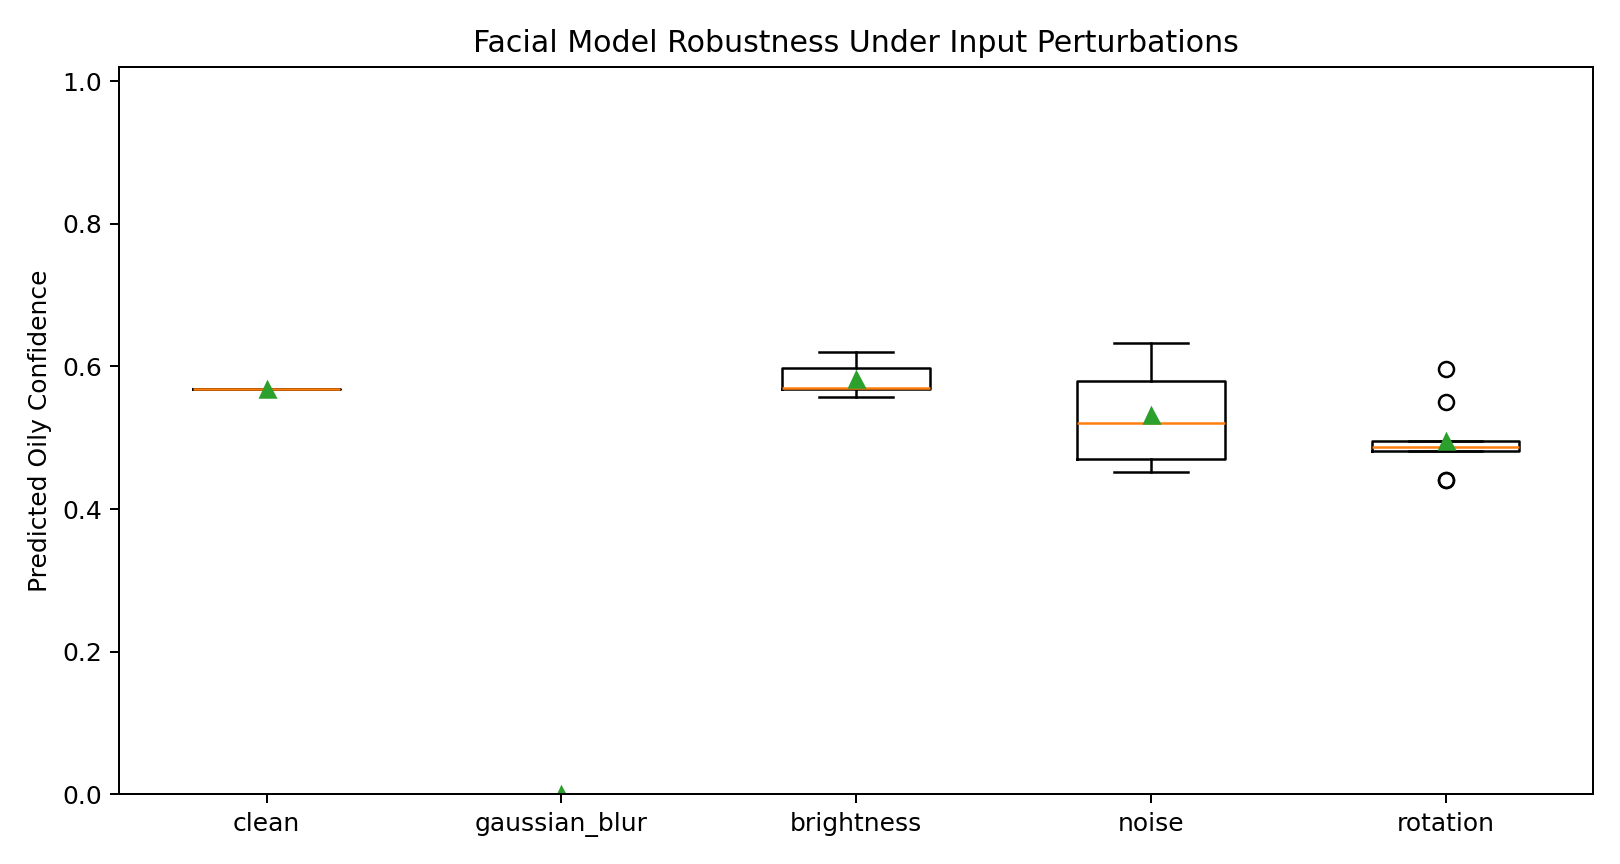
\includegraphics[width=0.92\linewidth]{figures/facial_robustness_confidence.png}
  \caption{Facial-model confidence robustness across controlled perturbations.}
  \label{fig:facial_robustness}
\end{figure}

\subsection{OCR Extraction Quality}
OCR quality was measured on 40 synthetic label images (10 each for clean, blurred, rotated, and noisy)
using exact normalized string matching against known ingredient sets.

\begin{table}[t]
\caption{OCR Quality by Image Condition}
\label{tbl:ocr_quality}
\begin{tabular*}{\tblwidth}{@{}LLLLL@{}}
\toprule
Condition & Samples & Precision & Recall & F1 \\
\midrule
Clean & 10 & 0.1871 & 0.1500 & 0.1655 \\
Blurred & 10 & 0.0000 & 0.0000 & 0.0000 \\
Rotated & 10 & 0.0310 & 0.0200 & 0.0243 \\
Noisy & 10 & 0.2990 & 0.2300 & 0.2585 \\
\midrule
Overall & 40 & 0.1293 & 0.1000 & 0.1121 \\
\bottomrule
\end{tabular*}
\end{table}

\begin{figure}[t]
  \centering
  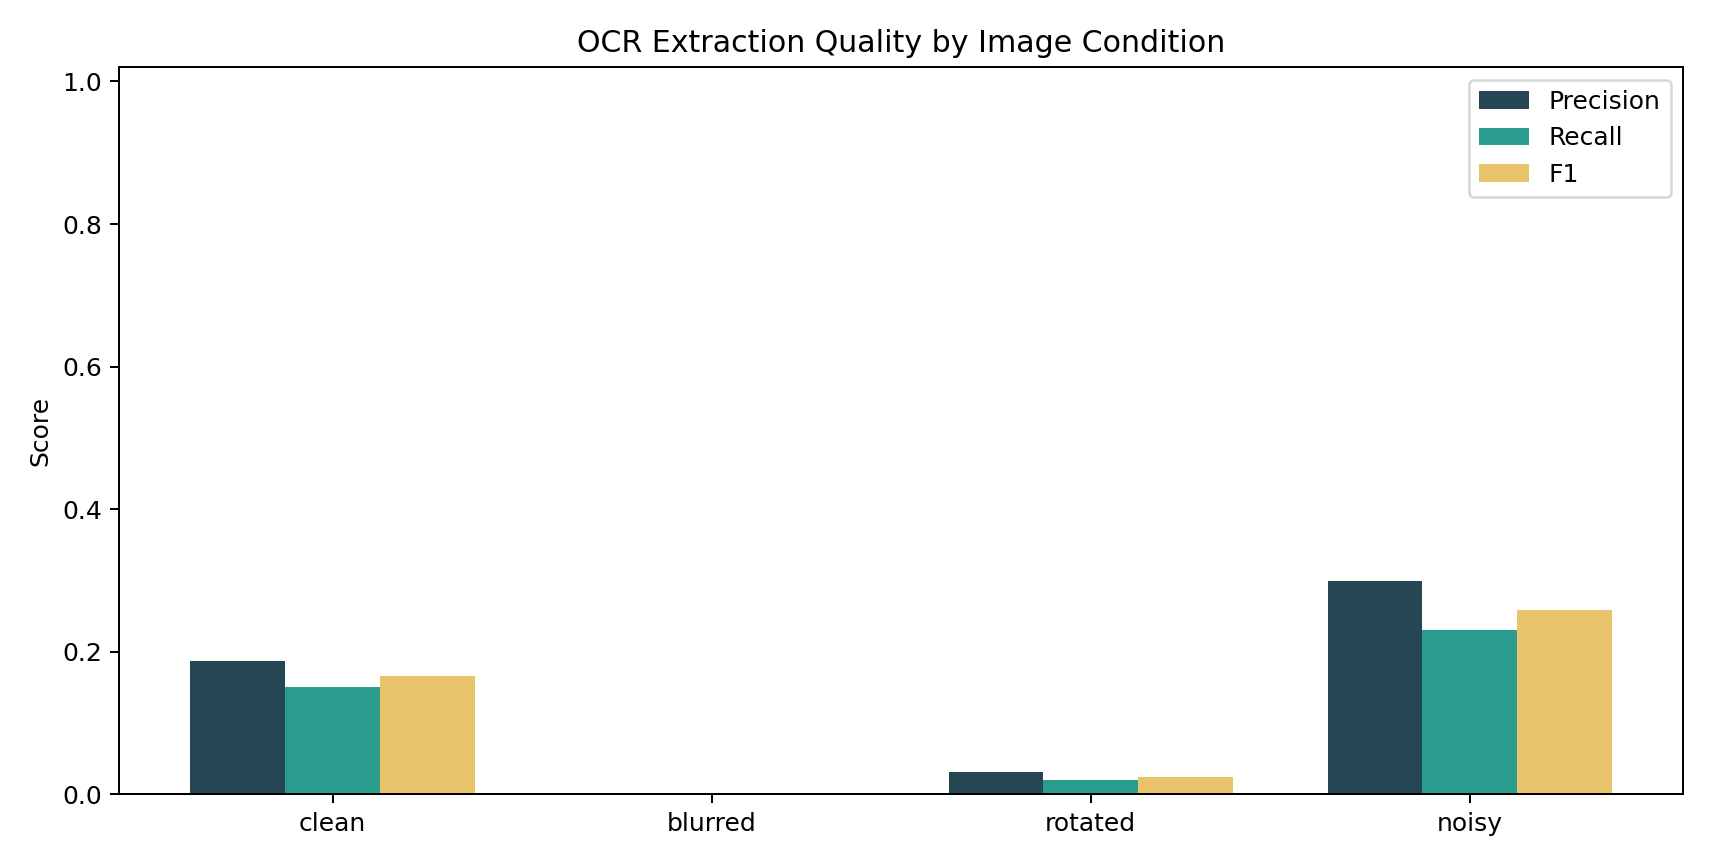
\includegraphics[width=0.92\linewidth]{figures/ocr_quality_by_condition.png}
  \caption{OCR precision, recall, and F1 under different image degradations.}
  \label{fig:ocr_quality}
\end{figure}

A real-image smoke check on \texttt{testing/dry\_moisturizer.jpg} returned 27 ingredients with high
confidence in 8669.3 ms. The low exact-match F1 in synthetic tests is mainly driven by strict string-level
matching and OCR spelling variance, not complete extraction failure.

\section{Comparative Analysis}\label{sec:comparison}
To compare candidate ML algorithms (XGBoost, Random Forest, Gradient Boosting, and others), we ran
controlled synthetic benchmarking with 2500 samples per task and identical train/validation splits.

\begin{table}[t]
\caption{Comparative Results: Single-Product Task (2500 Samples)}
\label{tbl:cmp_individual}
\begin{tabular*}{\tblwidth}{@{}LLLLL@{}}
\toprule
Model & MAE & RMSE & $R^2$ & Infer (\textmu s/sample) \\
\midrule
Linear Regression & 2.5086 & 3.0947 & 0.9462 & 1.82 \\
Random Forest & 2.6359 & 3.2256 & 0.9416 & 131.31 \\
Gradient Boosting (sklearn) & 2.6342 & 3.2522 & 0.9406 & 4.64 \\
XGBoost (SkinSpectra) & 2.8041 & 3.5265 & 0.9302 & 11.39 \\
SVR (RBF) & 3.4196 & 4.6154 & 0.8804 & 527.07 \\
KNN (k=5) & 5.9650 & 7.7089 & 0.6665 & 7093.66 \\
\bottomrule
\end{tabular*}
\end{table}

\begin{table}[t]
\caption{Comparative Results: Layering Task (2500 Samples)}
\label{tbl:cmp_layering}
\begin{tabular*}{\tblwidth}{@{}LLLLL@{}}
\toprule
Model & MAE & RMSE & $R^2$ & Infer (\textmu s/sample) \\
\midrule
Linear Regression & 2.8882 & 3.6573 & 0.9819 & 2.82 \\
Gradient Boosting (sklearn) & 2.9522 & 3.7114 & 0.9814 & 4.69 \\
Random Forest & 3.0532 & 3.9039 & 0.9794 & 119.33 \\
LightGBM (SkinSpectra) & 3.2474 & 4.0422 & 0.9779 & 36.98 \\
SVR (RBF) & 4.4937 & 6.0394 & 0.9507 & 562.24 \\
KNN (k=5) & 13.0445 & 15.4952 & 0.6757 & 49.21 \\
\bottomrule
\end{tabular*}
\end{table}

Figure~\ref{fig:model_comparison_r2} summarizes the comparative $R^2$ profile across both tasks.
Tree ensembles and linear models dominate error-based metrics, while KNN/SVR underperform in
latency-quality tradeoff.

\begin{figure}[t]
  \centering
  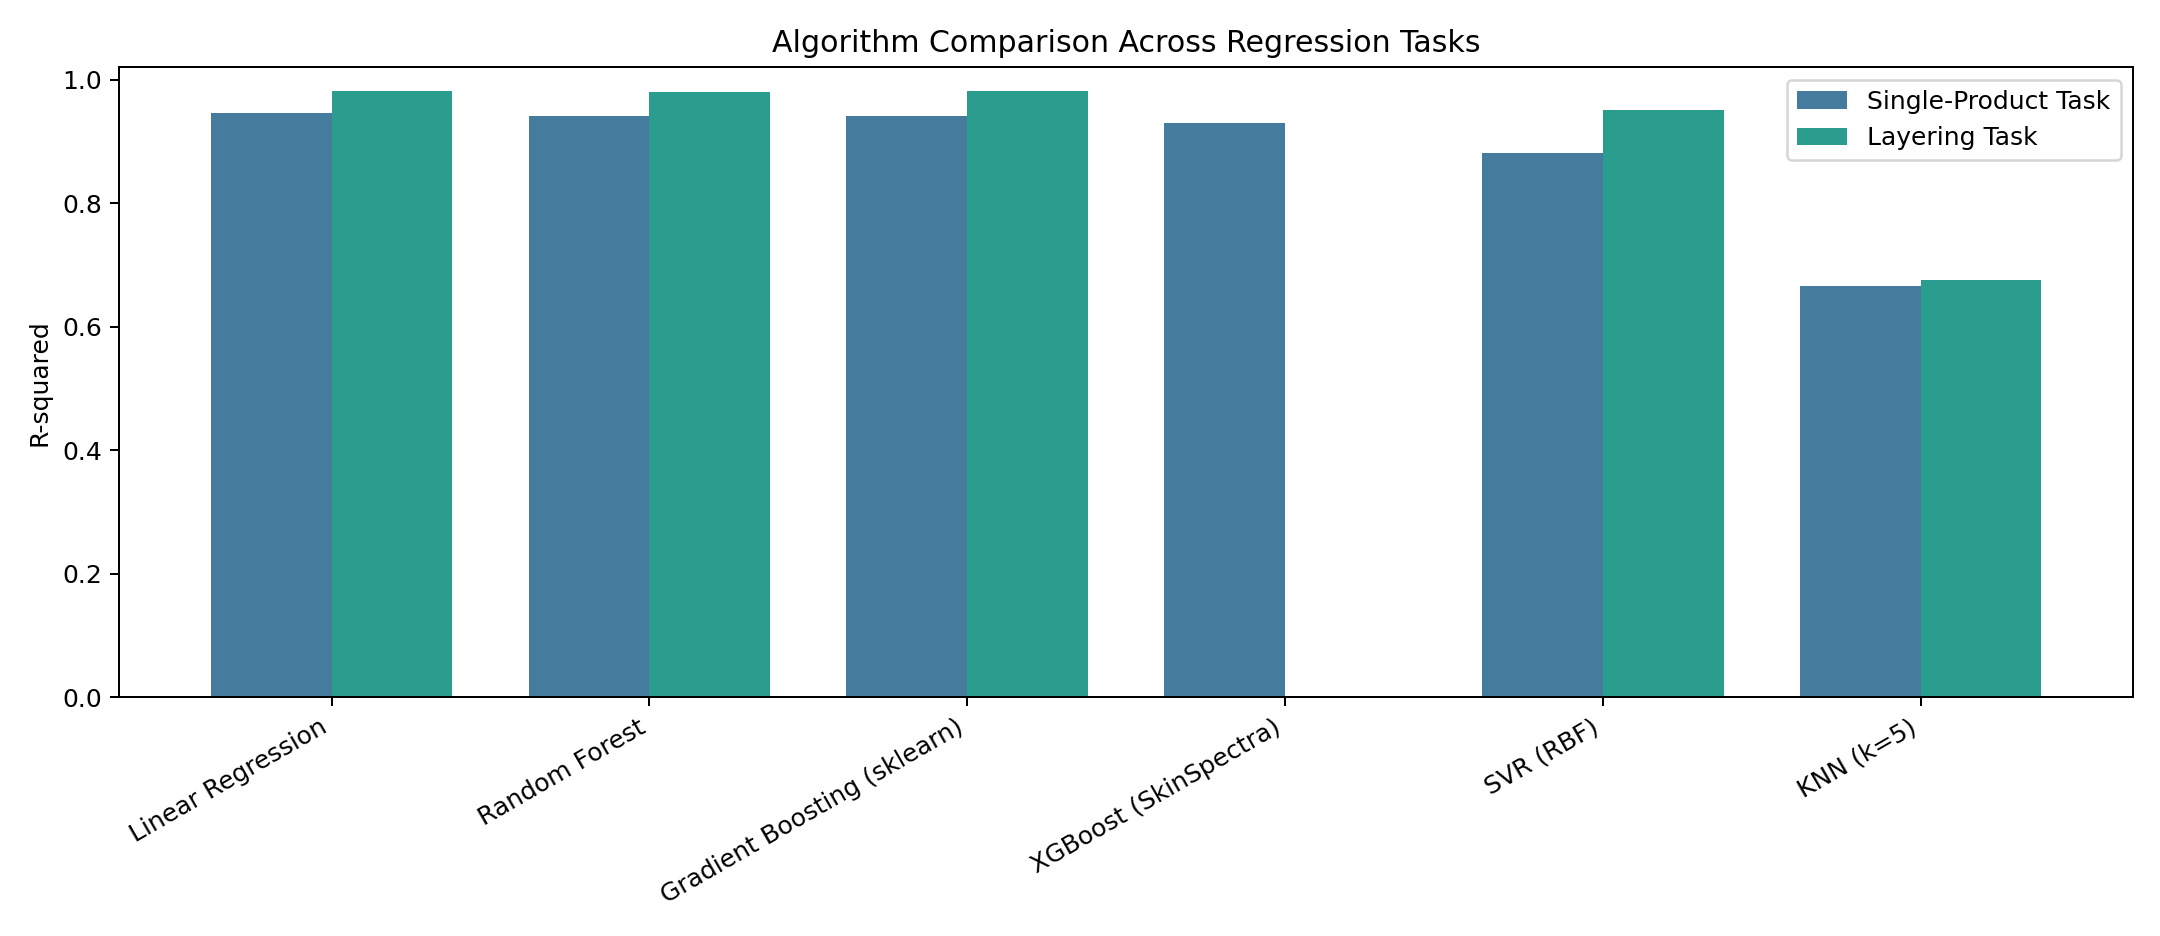
\includegraphics[width=0.98\linewidth]{figures/model_comparison_r2.png}
  \caption{$R^2$ comparison of candidate regressors for single-product and layering tasks.}
  \label{fig:model_comparison_r2}
\end{figure}

Compared with common consumer tools, SkinSpectra still provides broader practical utility by combining
NLP normalization, profile-aware scoring, interaction-aware layering logic, OCR intake, and optional LLM
explanations in one deployable API.

\section{Conclusion}\label{sec:conclusion}
SkinSpectra demonstrates that a multi-layer AI system can deliver robust, interpretable, and deployable skincare compatibility analysis. The project integrates heterogeneous methods without sacrificing API usability: semantic normalization for noisy ingredient inputs, high-quality regression for compatibility estimation, image-based extraction and skin-type support, and optional natural-language reporting grounded in computed scores.

Current model metrics validate the feasibility of the approach for CEP-level implementation. Future improvement directions include broader ingredient coverage, richer conflict datasets, formal comparative retraining across additional baseline regressors, and expanded benchmark reporting for throughput and latency under production-like load.

\section{Acknowledgment}\label{sec:ack}
This report was prepared for the SE-412 Artificial Intelligence course as a Complex Engineering Problem submission. The authors acknowledge open-source ecosystems including FastAPI, scikit-learn, XGBoost, LightGBM, TensorFlow/Keras, and sentence-transformers.

% Numbered list
% Use the style of numbering in square brackets.
% If nothing is used, default style will be taken.
%\begin{enumerate}[a)]
%\item 
%\item 
%\item 
%\end{enumerate}  

% Unnumbered list
%\begin{itemize}
%\item 
%\item 
%\item 
%\end{itemize}  

% Description list
%\begin{description}
%\item[]
%\item[] 
%\item[] 
%\end{description}  

\clearpage %%Remove this from your manuscript

% Uncomment and use as the case may be
%\begin{theorem} 
%\end{theorem}

% Uncomment and use as the case may be
%\begin{lemma} 
%\end{lemma}

%% The Appendices part is started with the command \appendix;
%% appendix sections are then done as normal sections
%% \appendix

\section{Ethical and Practical Scope}\label{sec:scope}
SkinSpectra is an assistive software system for skincare guidance and not a medical diagnosis platform. Users with persistent or severe dermatological conditions should consult certified dermatologists. The system prioritizes conservative warnings for pregnancy and high-irritancy combinations.

% To print the credit authorship contribution details
\printcredits

%% Loading bibliography style file
%\bibliographystyle{model1-num-names}
\bibliographystyle{cas-model2-names}

% Loading bibliography database
\bibliography{cas-refs}

% Biography
%\bio{}
% Here goes the biography details.
%\endbio

%\bio{pic1}
% Here goes the biography details.
%\endbio

\end{document}

